\documentclass[journal]{IEEEtran}
\usepackage[T1]{fontenc}
\usepackage[utf8]{inputenc}
\usepackage[polish]{babel}
\usepackage{graphicx}
\pagestyle{plain}
\setlength{\parskip}{0.7em}  
\setlength{\parindent}{15pt}


\ifCLASSINFOpdf
  
\else
 
\fi





% correct bad hyphenation here
\hyphenation{op-tical net-works semi-conduc-tor}


\begin{document}

\title{Ocena zmienności rytmu serca w oparciu o uczenie maszynowe}
\author{
    J. Bancerewicz, J. Kotłowski, O. Lozovyy, J. Morawska, M. Rzęsa\\
    \textit{Politechnika Gdańska}\\
    \textit{Wydział Elektroniki, Telekomunikacji i Informatyki}
}


% The paper headers
\markboth{}%
{Shell \MakeLowercase{\textit{et al.}}: Bare Demo of IEEEtran.cls for IEEE Journals}
\maketitle


% Note that keywords are not normally used for peerreview papers.
%\begin{IEEEkeywords}
%IEEE, IEEEtran, journal, \LaTeX, paper, template.
%\end{IEEEkeywords}

\IEEEpeerreviewmaketitle



\section{Wstęp}

%\IEEEPARstart{T}{his} demo file is intended to serve as a ``starter file''
%for IEEE journal papers produced under \LaTeX\ using
%IEEEtran.cls version 1.8b and later.

\newpage
\section{Przegląd metod z użyciem uczenia maszynowego}

Metody uczenia maszynowego znajdują szerokie zastosowanie w przetwarzaniu sygnałów biomedycznych, w tym w elektrokardiografii oraz fotopletyzmografii. Techniki te umożliwiają automatyczną detekcję istotnych cech, ocenę długotrwałych zależności czasowych oraz szacowanie parametrów fizjologicznych. W literaturze wyróżnia się dwa główne podejścia: metody oparte na filtracji sygnałów i analizie w dziedzinie czasu oraz modele uczące się, zdolne do samodzielnego wyodrębniania wzorców z danych pomiarowych.

Analiza sygnałów elektrokardiograficznych coraz częściej wykorzystuje metody uczenia maszynowego, jak sieci splotowe czy rekurencyjne, ze względu na możliwość detekcji złożonych zależności czasowych. W związku z wysoką odpornością na szumy i zakłócenia modele ML implementowane są do automatycznej detekcji załamków R. W opracowaniach opisywane są również klasyczne metody, takie jak filtry progowe czy transformacje sygnału. Ich zastosowanie w warunkach rzeczywistych jest utrudnione spadkiem efektywności w obecności zniekształceń ruchowych. W odpowiedzi na ograniczenia, modele głębokiego uczenia stanowią alternatywę dla standardowych metod analizy danych \cite{1}.

Algorytm Pan-Tompkins, szeroko stosowany w przetwarzaniu EKG, wykazuje ograniczoną skuteczność przy niskiej jakości danych. Zaawansowane metody wykorzystują architektury splotowe do ekstrakcji lokalnych cech sygnału oraz sieci rekurencyjne do detekcji zależności czasowych, opisujących relacje między kolejnymi interwałami RR, istotnych dla analizy zmienności rytmu serca \cite{2}. Natomiast modele Transformer umożliwiają jednoczesną identyfikację dynamiki zapisu, zwiększając jego odporność na zakłócenia.  Architektury hybrydowe łączące sieci CNN i RNN osiągają wyższą skuteczność w klasyfikacji nieregularnych przebiegów EKG oraz poprawiają dokładność analizy HRV, jednocześnie minimalizując wady pojedynczych rozwiązań \cite{3}.

\newpage
Analogicznie do sygnałów elektrokardiograficznych, w fotopletyzmografii obserwuje się wykorzystanie algorytmów uczenia maszynowego w monitorowaniu i analizie częstości pracy serca. Wysoka podatność zapisu PPG na zakłócenia ruchowe oraz zmiany oświetlenia ogranicza skuteczność metod filtracji i detekcji. Zastosowanie uczenia głębokiego umożliwia precyzyjne wykrywanie szczytów fali, poprawiając wiarygodność klasyfikacji \cite{4}.

W przetwarzaniu sygnałów PPG wykorzystuje się filtrację pasmową oraz algorytmy detekcji lokalnych maksimów i progów, uwzględniające adaptację do zmian amplitudy. Pomimo wysokiej skuteczności w warunkach kontrolowanych, metody te charakteryzują się obniżoną efektywnością w obecności nasilonych zakłóceń. W nowoczesnej analizie stosuje się architektury głębokiego uczenia, w których warstwy konwolucyjne łączone są z rekurencyjnymi LSTM umożliwiając modelowanie zarówno krótkookresowych, jak i długoterminowych zmian przebiegu fali \cite{5}. W procesie klasyfikacji wyodrębnionych cech implementuje się również wielowarstwowe perceptrony MLP oraz sieci GRU, które przy mniejszej liczbie parametrów wykrywają zależności czasowe z dokładnością zbliżoną do architektury LSTM.
Z sygnału PPG wyznacza się interwały międzyuderzeniowe IBI, odpowiadające interwałom RR w EKG, pozwalając na analizę zmienności rytmu serca niezależnie od zapisów elektrokardiograficznych. W wybranych rozwiązaniach wykorzystuje się uczenie transferowe, umożliwiające dostosowanie modeli wytrenowanych na odmiennych zbiorach danych, zapewniając wyższą precyzję detekcji oraz odporność na zakłócenia \cite{6}.


\subsection{Elektrokardiografia}
Jednym z elementów zaprojektowanych w ramach niniejszej pracy jest sieć łącząca warstwy splotowe oraz rekurencyjne, przeznaczoną do rozpoznawania szczytów R w sygnale EKG. Stanowi ona pierwszy etap w procesie wyznaczania interwałów RR oraz parametrów zmienności rytmu serca.

Model przetwarza jednowymiarowe sygnały napięcia elektrycznego, podzielone na fragmenty o długości 256 próbek. Moduły splotowe odpowiadają za ekstrakcję cech z danych wejściowych przez zastosowanie kolejnych warstw konwolucyjnych wraz z nieliniowymi funkcjami aktywacji. Realizacja procesu redukcji wymiarowości przez wybór największych wartości pozwala na zwiększenie odporności na szum oraz zakłócenia. Po przekształceniu sygnału przez część konwolucyjną, dane przekazywane są do jednokierunkowej warstwy LSTM, umożliwiającej analizę zależności czasowych między kolejnymi próbkami sygnału. W końcowej części modelu wykorzystano połączone moduły liniowe, których celem jest konwersja wewnętrznych cech w przestrzeń logitów. Każdy element wektora reprezentuje prawdopodobieństwo wystąpienia załamka R w odpowiadającej mu próbce sygnału wejściowego. Zaprojektowane rozwiązanie umożliwia binarną klasyfikację dla każdego punktu czasowego.

\newpage
Model został wytrenowany w trybie nadzorowanym na podstawie sygnałów pochodzących z czujnika tętna Polar H10. Dla danych treningowych wykorzystano funkcję ecg\_peaks z biblioteki NeuroKit2, implementującą algorytm Pan–Tompkins, umożliwiający detekcję załamków R w przefiltrowanym zapisie EKG. Dla każdej próbki przygotowano etykiety binarne wskazujące obecność lub brak lokalnego maksimum. W konsekwencji sieć neuronowa uczyła się klasyfikacji poprzez identyfikację wzorców odpowiadającym rzeczywistym szczytom R.


\subsection{Fotopletyzmografia}
Drugim opracowanym rozwiązaniem jest sieć wykorzystująca warstwy splotowe, przeznaczona do analizy sygnału fotopletyzmograficznego. Model ten odpowiada za detekcję lokalnych szczytów, na podstawie których wyznaczane są interwały międzyuderzeniowe, służące do szacowania wskaźników rytmu serca.

System przetwarza jednowymiarowe sygnały reprezentujące zmiany objętości krwi w naczyniach obwodowych, podzielone na segmenty o długości 50 próbek. Kolejne moduły splotowe, wykorzystujące nieliniowe funkcje aktywacji, odpowiadają za identyfikację lokalnych wzorców w danych wejściowych. Selekcja wartości o największej amplitudzie zwiększa odporność na niepożądane zakłócenia. Na wyjściu modelu generowany jest wektor prawdopodobieństw, otrzymany przez zastosowanie funkcji sigmoidalnej do surowych sygnałów warstwy konwolucyjnej. Uzyskane wartości odzwierciedlają lokalizacje szczytów fali, umożliwiając klasyfikację binarną próbek w reprezentacji czasowej.


Uczenie nadzorowane, zastosowane w analizie sygnału EKG pozyskanego z pulsometru, zostało analogicznie zaimplementowane dla danych PPG rejestrowanych za pomocą urządzenia mobilnego. Proces etykietowania oparto na identyfikacji szczytów lokalnych, wykorzystując funkcję find\_peaks z modułu scipy.signal, w przefiltrowanym przebiegu. Każdej próbce przypisano wartość binarną, odzwierciedlającą obecność bądź brak piku fali. Na podstawie zdefiniowanych etykiet sieć neuronowa została wytrenowana do rozpoznawania wzorców odpowiadających detekcji szczytów.

\newpage
\section{Opis systemu i danych}
\subsection{Akwizycja danych}
\subsubsection{Akwizycja danych EKG}
Dane wykorzystane do trenowania i walidacji modelu detekcji załamków R zostały pozyskane za pomocą pulsometru Polar H10, zdolnego do rejestrowania sygnału elektrokardiograficznego z częstotliwością próbkowania wynoszącą 130 Hz. Przyjęta wartość umożliwia charakterystykę przebiegu sygnału istotną dla oceny aktywności serca oraz analizę zmienności rytmu zatokowego.

W celu zgromadzenia odpowiedniego zbioru danych przeprowadzono dwugodzinne eksperymenty pomiarowe z udziałem pięciu osób. Rejestrowane przebiegi były zróżnicowane pod względem poziomu aktywności fizycznej, zmienności rytmu serca, a także obecnością nagłych ruchów ciała, mogących wprowadzać zakłócenia w sygnale.

Transmisja danych między czujnikiem a komputerem zrealizowano bezprzewodowo z wykorzystaniem technologii Bluetooth Low Energy. Dane przesyłano w czasie rzeczywistym w pakietach zawierających 13 próbek, zgodnych z zastosowaną częstotliwością próbkowania, a następnie zapisywano je w formacie CSV. Każdy odczyt odpowiadał wartości potencjału elektrycznego rejestrowanego z powierzchni klatki piersiowej użytkownika.

\subsubsection{Akwizycja danych PPG}
Dane wykorzystane do trenowania i walidacji modelu detekcji szczytów fali zostały pozyskane przy użyciu tylnej kamery smartfona z systemem Android. Rejestrację sygnału fotopletyzmograficznego przeprowadzono poprzez umieszczenie opuszka palca bezpośrednio na obiektywie kamery oraz zintegrowanym źródle światła LED. Przyjęte ustawienie umożliwiło transmisję światła przez tkanki skórne i zapis zmian optycznych wywołanych cyklicznymi wahaniami objętości krwi. Obrazy przechwytywano w czasie rzeczywistym w formacie YUV 4:2:0 o rozdzielczości 640×480. Z każdej klatki wyodrębniano składową luminancji, na podstawie której obliczano średnią wartość jasności pikseli. Otrzymana wartość stanowiła pojedynczą próbkę surowego sygnału fotopletyzmograficznego.

W celu zgromadzenia odpowiedniego zbioru danych zrealizowano serię pomiarów z udziałem sześciu osób. Każda sesja trwała 10 minut i obejmowała rejestrację sygnału w zróżnicowanych warunkach, uwzględniających drobne ruchy palca wpływające na zmienność przepływu krwi.

Transmisja danych pomiędzy smartfonem a komputerem zrealizowano z wykorzystaniem protokołu WebSocket. Informacje przesyłano w pakietach zawierających pojedyncze próbki sygnału wraz z odpowiadającymi im znacznikami czasu. Częstotliwość próbkowania była zgodna z liczbą klatek wideo, wynoszącą około 30 Hz. Odebrane dane buforowano na komputerze i zapisywane w formacie CSV.

\subsection{Filtracja sygnału – filtr Butterwortha}
Do przetwarzania sygnału EKG wykorzystano cyfrowy filtr Butterwortha piątego rzędu o charakterystyce pasmowo-przepustowej, obejmującej zakres częstotliwości od 0,5 Hz do 45 Hz, mający na celu eliminację szumów oraz zakłóceń. Dolna granica pasma redukuje powolne zmiany w sygnale wywołane ruchem ciała lub niestabliną pozycją elektrod  \cite{7}. Z kolei górna tłumi zakłócenia sieciowe, elektromagnetyczne oraz mięśniowe  \cite{8}. Filtracja danych została przeprowadzona przy użyciu funkcji nk.signal\_filter z biblioteki NeuroKit2.

\begin{figure}[htbp]
    \centering
    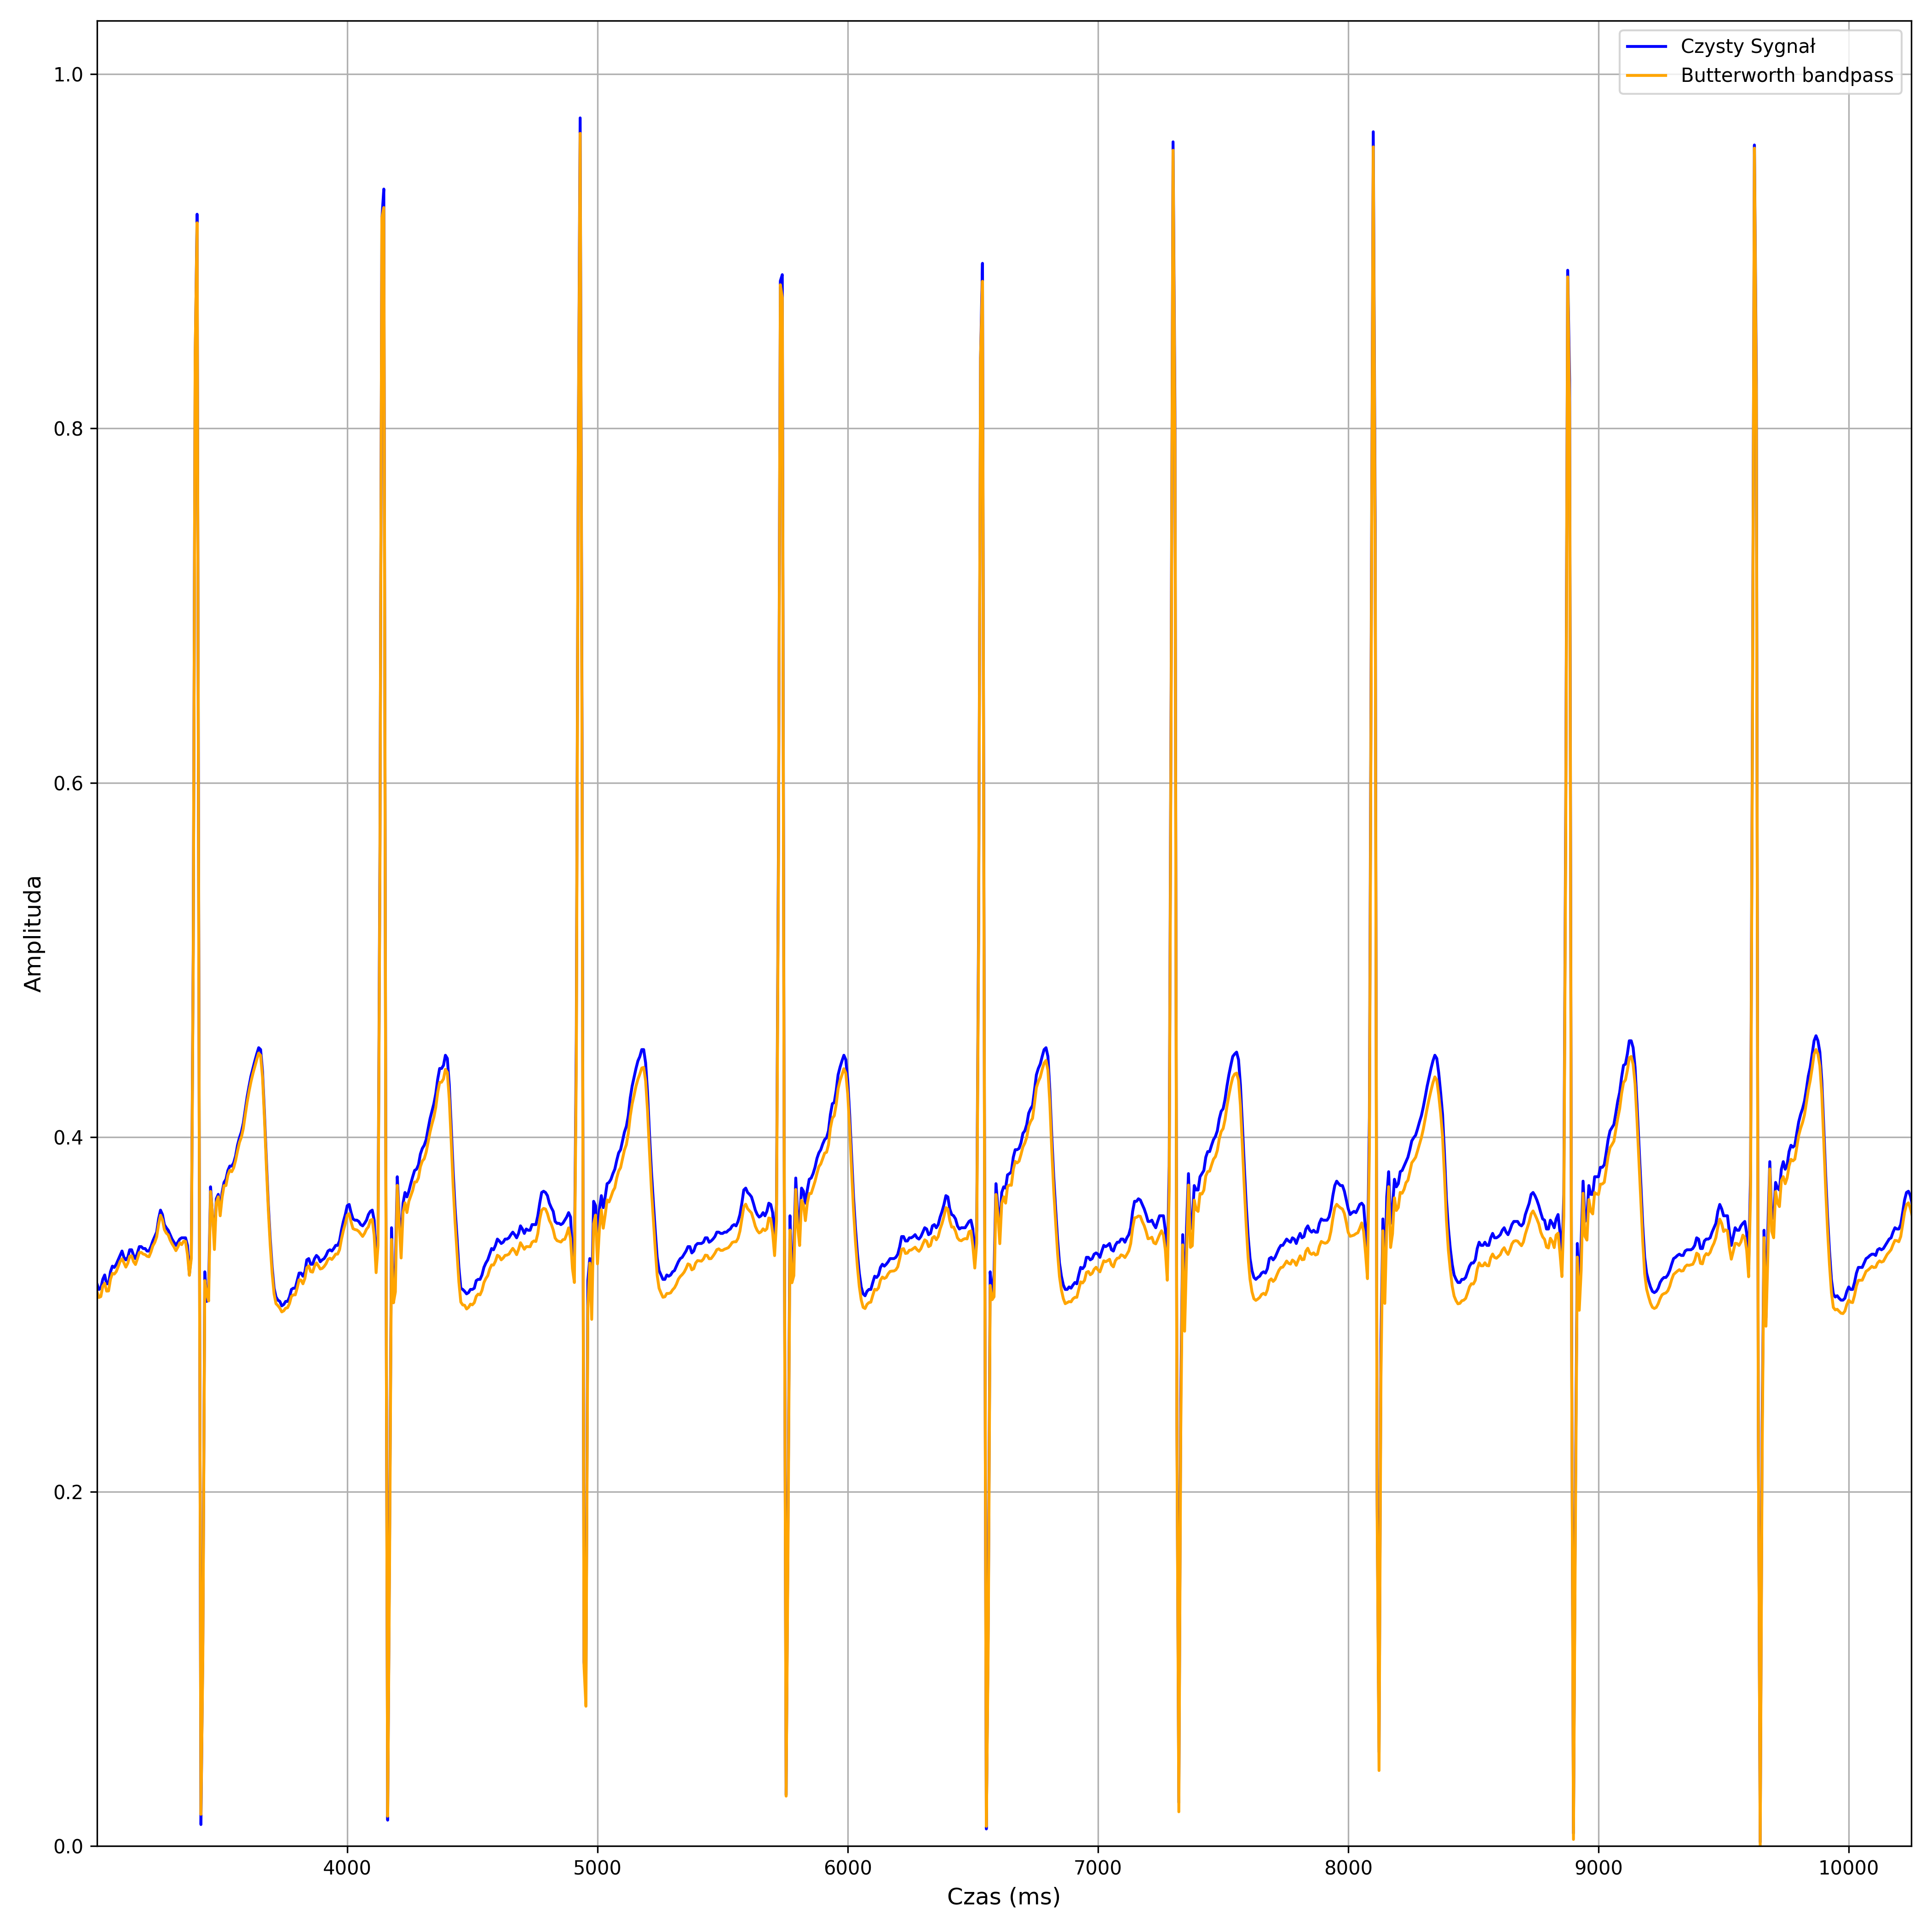
\includegraphics[width=0.76\linewidth]{Filtr_EKG.png} 
    \caption{Porównanie surowego i przefiltrowanego sygnału EKG}
    \label{fig:filtr_ekg}
\end{figure}

W celu poprawy jakości sygnału PPG wykorzystano cyfrowy filtr Butterwortha czwartego rzędu, działający w zakresie 0,5–5 Hz. Dolna granica pasma ogranicza zakłócenia spowodowane ruchem ciała czy niestabilnym kontaktem czujnika ze skórą, natomiast górna tłumi szumy urządzenia pomiarowego i interferencje optyczne  \cite{9}. Filtracja została zrealizowana z wykorzystaniem funkcji butter oraz filtfilt z modułu scipy.signal, zapewniając obróbkę sygnału bez przesunięcia fazowego.

\begin{figure}[htbp]
    \centering
    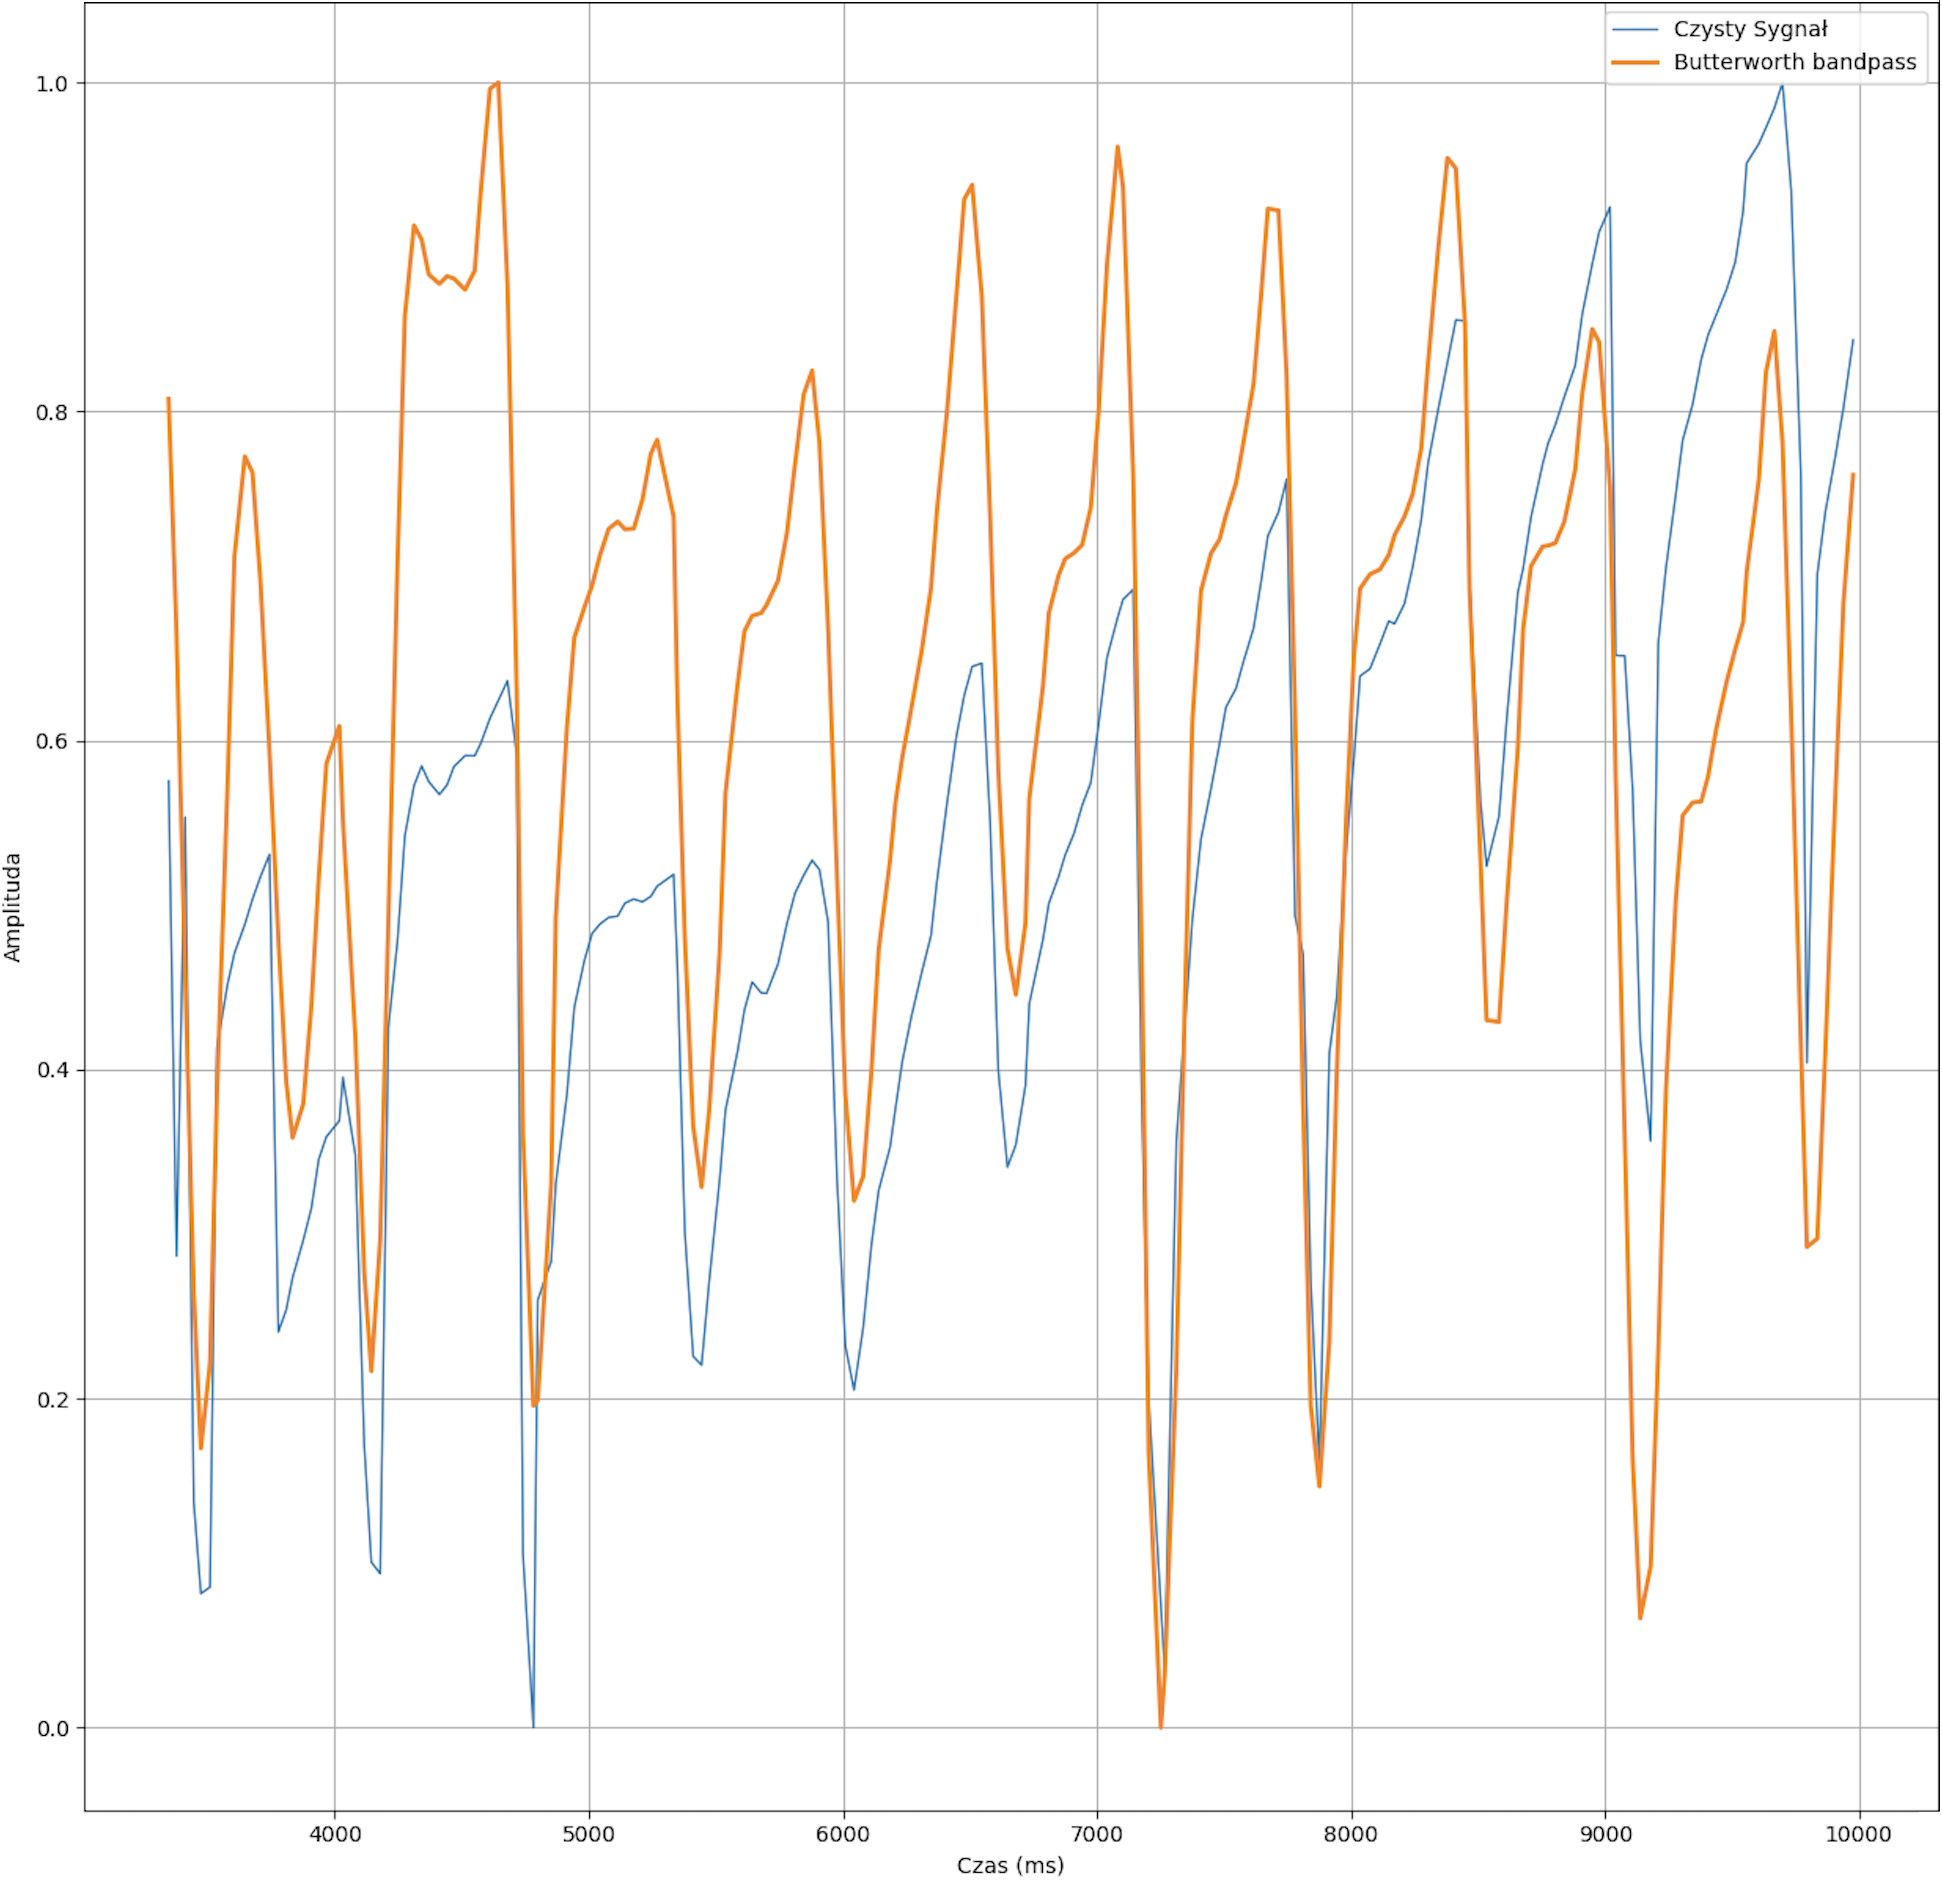
\includegraphics[width=0.76\linewidth]{Filtr_PPG.png} 
    \caption{Porównanie surowego i przefiltrowanego sygnału PPG}
    \label{fig:filtr_ppg}
\end{figure}

\newpage
\subsection{Modele detekcji}
\subsubsection{Model do wykrywania załamków R}
Sieć neuronowa została zaimplementowana z wykorzystaniem biblioteki PyTorch. Architektura składa się z czterech warstw splotowych typu 1D, jednokierunkowej warstwy LSTM oraz bloków dwóch warstw liniowych. Sygnał wejściowy ma postać jednowymiarowej sekwencji o wymiarach [1 × 256], zawierającą 256 próbek w pojedynczym kanale.

Pierwszy etap obejmuje ekstrakcję cech przy użyciu czterech warstw konwolucyjnych 1D, których parametry zestawiono w Tabeli~\ref{tab:conv_layers}. Warstwy te rozszerzają reprezentację sygnału, zwiększając liczbę kanałów od 16 do 128, wykorzystując filtry o rozmiarach 5 lub 3. Dla każdego przekształcenia zastosowano normalizację BatchNorm1d oraz nieliniową funkcję aktywacji LeakyReLU. Maksymalne próbkowanie MaxPooling1D z jądrem o rozmiarze 2 redukuje długość sekwencji z 256 do 16 wzdłuż osi czasowej, zwiększając efektywność przetwarzania.

Macierz danych o wymiarach [128 × 16] jest przekształcana przez jednokierunkową LSTM z 128 jednostkami ukrytymi, działającą w trybie batch\_first=True. Otrzymany wektor został spłaszczony i przekazany do warstwy z 128 neuronami, a następnie do końcowego bloku zawierającego 256 elementów, odwzorowującego kolejne próbki sygnału wejściowego. Każdy logit w wektorze reprezentuje miarę pewności modelu dotyczącą obecności piku R w danej próbce.

Trening modelu przeprowadzono w trybie nadzorowanym, w partiach po 32 próbki, z wykorzystaniem funkcji straty BCEWithLogitsLoss, umożliwiającej binarną klasyfikację sygnału. Do optymalizacji zastosowano algorytm Adam przy stałej wartości współczynnika uczenia wynoszącej 0,0001.

\begin{table}[h!]
\centering
\caption{Parametry warstw konwolucyjnych sieci}
\label{tab:conv_layers}
\begin{tabular}{|l|c|c|c|c|c|}
\hline
\textbf{Warstwa} & \textbf{Wejście} & \textbf{Wyjście} & \textbf{Filtr} & \textbf{Padding} & \textbf{Aktywacja} \\
\hline
Conv1D-1 & 1   & 16  & 5 & 2 & LReLU+BN \\
Conv1D-2 & 16  & 32  & 5 & 2 & LReLU+BN \\
Conv1D-3 & 32  & 64  & 3 & 1 & LReLU+BN \\
Conv1D-4 & 64  & 128 & 3 & 1 & LReLU+BN \\
\hline
\end{tabular}
\end{table}

Efektywność zaprojektowanej sieci neuronowej oceniono na podstawie wyników uzyskanych na niezależnym zbiorze danych, wykorzystując wytrenowane parametry modelu. Rezultaty klasyfikacji przedstawiono w postaci macierzy konfuzji w Tabeli~\ref{tab:conf_matrix}.

\begin{table}[ht]
\centering
\caption{Macierz konfuzji dla detekcji załamków R}
\label{tab:conf_matrix}
\begin{tabular}{|c|c|c|}
\hline
\textbf{Rzeczywiste / Predykcja} & \textbf{Brak szczytu } & \textbf{Szczyt } \\
\hline
Brak szczytu  & 231170 & 53 \\
\hline
Szczyt  & 83 & 2678 \\
\hline
\end{tabular}
\end{table}

\newpage
Model poprawnie zaklasyfikował 231170 próbek niezawierających piku R oraz 2678 z jego rzeczywistą obecnością. Liczba fałszywie pozytywnych predykcji wyniosła 53, natomiast fałszywie negatywnych -- 83. Wartość miary F1 równa 0,9753 świadczy o wysokiej równowadze pomiędzy precyzją a czułością modelu, co jest kluczowe w automatycznej analizie sygnałów elektrokardiograficznych. Podstawowe metryki oceny jakości modelu przedstawiono w Tabeli~\ref{tab:metrics}.

\begin{table}[ht]
\centering
\caption{Parametry detekcji szczytów R}
\label{tab:metrics}
\begin{tabular}{|c|c|p{4.6cm}|}
\hline
\textbf{Metryka} & \textbf{Wartość} & \textbf{Opis} \\
\hline
Skuteczność & 96,99\% & Odsetek poprawnych klasyfikacji obecności lub braku piku R. \\
\hline
Błędne detekcje & 0,00\% & Odsetek próbek fałszywie zaklasyfikowanych jako zawierające pik R. \\
\hline
Pominięte załamki & 3,01\% & Odsetek próbek z niewykrytym rzeczywistym pikiem R. \\
\hline
\end{tabular}
\end{table}

\subsubsection{Model do wykrywania szczytów fali}
Analogicznie do podejścia zastosowanego w detekcji załamków R w sygnale EKG, opracowano model do identyfikacji szczytów w przebiegu fotopletyzmograficznym, wykorzystujący bibliotekę PyTorch. Sieć opiera się na strukturze trzech warstw konwolucyjnych 1D, przetwarzającej dane w postaci wektora o wymiarach [1 × 50], zawierającego 50 próbek w pojedynczym kanale.

Do ekstrakcji lokalnych cech zastosowano dwie warstwy konwolucyjne 1D z filtrami o szerokości 5 oraz rosnącą liczbą kanałów od 1 do 32. Każde z przekształceń obejmuje normalizację BatchNorm1d oraz nieliniową funkcję aktywacji ReLU. Końcowy blok z filtrem o rozmiarze 1 generuje jednowymiarowy wektor, którego wartości wyznaczane przez funkcję sigmoidalną odpowiadają prawdopodobieństwom wystąpienia szczytu w danej próbce sygnału. Szczegółowe parametry warstw splotowych uwzględniono w Tabeli~\ref{tab:ppg_layers}.

Model trenowano w trybie nadzorowanym, w partiach po 32 próbki, z wykorzystaniem funkcji straty BCELoss, odpowiedniej do binarnej klasyfikacji sygnałów. Do optymalizacji zastosowano algorytm Adam przy stałej wartości współczynnika uczenia wynoszącej 0,001.

\begin{table}[ht]
\centering
\caption{Parametry warstw konwolucyjnych sieci}
\label{tab:ppg_layers}
\begin{tabular}{|l|c|c|c|c|c|}
\hline
\textbf{Warstwa} & \textbf{Wejście} & \textbf{Wyjście} & \textbf{Filtr} & \textbf{Padding} & \textbf{Aktywacja} \\
\hline
Conv1D-1 & 1 & 16 & 5 & 2 & ReLU+BN \\
Conv1D-2 & 16 & 32 & 5 & 2 & ReLU+BN \\
Conv1D-3 & 32 & 1 & 1 & 0 & Sigmoid \\
\hline
\end{tabular}
\end{table}

\newpage
Skuteczność zaprojektowanego modelu oceniono na podstawie wyników uzyskanych na niezależnym zbiorze danych, przy użyciu wcześniej wytrenowanych parametrów. Wyniki klasyfikacji przedstawiono w formie macierzy konfuzji w Tabeli~\ref{tab:conf_matrix_ppg}.

\begin{table}[ht]
\centering
\caption{Macierz konfuzji dla detekcji pików fali}
\label{tab:conf_matrix_ppg}
\begin{tabular}{|c|c|c|}
\hline
\textbf{Rzeczywiste / Predykcja} & \textbf{Brak szczytu } & \textbf{Szczyt} \\
\hline
Brak szczytu  & 9610 & 8 \\
\hline
Szczyt  & 12 & 370 \\
\hline
\end{tabular}
\end{table}

Dla sygnałów fotopletyzmograficznych model poprawnie rozpoznał 9610 próbek bez obecności fali oraz 370 z jej wystąpieniem. Niepoprawne predykcje odnotowano w 8 przypadkach fałszywie dodatnich oraz 12  fałszywie ujemnych. Otrzymana wartość miary F1, wynosząca 0,9737, jest zbliżona do wyników uzyskanych dla modelu EKG, potwierdzając wiarygodność zastosowanego rozwiązania w analizie obu typów sygnałów.
Podstawowe metryki oceny jakości architektury przedstawiono w Tabeli~\ref{tab:metrics_ppg}.

\begin{table}[ht]
\centering
\caption{Parametry detekcji szczytów fali}
\label{tab:metrics_ppg}
\begin{tabular}{|c|c|p{4.6cm}|}
\hline
\textbf{Metryka} & \textbf{Wartość} & \textbf{Opis} \\
\hline
Skuteczność & 97,12\% & Odsetek poprawnych klasyfikacji obecności lub braku piku fali. \\
\hline
Błędne detekcje & 0,00\% & Odsetek próbek fałszywie zaklasyfikowanych jako zawierające pik fali. \\
\hline
Pominięte załamki & 2,88\% & Odsetek próbek z niewykrytym rzeczywistym pikiem fali. \\
\hline
\end{tabular}
\end{table}

\section{Synchronizacja czasowa i analiza porównawcza parametrów HRV}

\subsection{Synchronizacja czasowa sygnałów}
Podczas rejestracji sygnałów EKG i PPG wykorzystywane są różne schematy zapisu znaczników czasowych. W elektrokardiogramie punkty wystąpienia załamków R początkowo określane są względem chwili rozpoczęcia akwizycji i zapisywane w sekundach jako czas względny. Podczas przetwarzania danych wartości te przekształcane są do formatu absolutnego UNIX, umożliwiając porównanie z przebiegiem PPG. W fotopletyzmografii detekcja szczytów fali rejestrowana jest bezpośrednio w czasie systemowym.

Dla ujednolicenia układu czasowego przekształca się dane EKG z czasu względnego na znaczniki UNIX, zgodnie z równaniem (1):
\begin{equation}
t_{\mathrm{UNIX}} = t_{\mathrm{rel}} + t_{0},
\end{equation}
gdzie $t_{\mathrm{UNIX}}$ - czas w formacie UNIX, $t_{\mathrm{rel}}$ – czas względny, a $t_{0}$ – początek akwizycji.

\newpage
Przebiegi zostały przedstawione w jednej osi czasu, umożliwiając ich automatyczną synchronizację. Różnice między odpowiadającymi pikami wyznaczono zgodnie z równaniem (2):
\begin{equation}
PTT = t_{\mathrm{PPG}} - t_{\mathrm{ECG}},
\end{equation}
gdzie $t_{\mathrm{PPG}}$, $t_{\mathrm{ECG}}$ - momenty detekcji szczytów w sygnale PPG i EKG. 

%Wskaźnik PTT wykorzystywany jest do oceny poprawności synchronizacji sygnałów.%

\subsection{Wskaźniki HRV}
Ujednolicenie osi czasowych umożliwia równoległą analizę odstępów kolejnych uderzeń serca w obu przebiegach. Dla sygnału EKG określa się interwały RR, odpowiadające odległościom między załamkami R, natomiast w PPG interwały międzyuderzenowe IBI. Na podstawie tych wartości wyznaczono standardowe parametry HRV, przedstawione w formie RR. Analogiczne obliczenia przeprowadzono dla odstępów IBI.

\noindent\textit{1) Średnia długość interwału:} 
Średnia arytmetyczna odstępów RR, wyrażona wzorem (3):
\begin{equation}
    Mean = \frac{1}{N} \sum_{i=1}^{N} RR_i
\end{equation}
gdzie $RR_i$ -- $i$-ty odstęp RR, a $N$ – liczba analizowanych odstępów.

\noindent\textit{2) Odchylenie standardowe odstępów NN:} 
Wielkość całkowitej zmienności rytmu serca, obliczana na podstawie wszystkich interwałów RR, wyrażona wzorem (4):
\begin{equation}
    SDNN = \sqrt{\frac{1}{N-1} \sum_{i=1}^{N} (RR_i - Mean)^2}
\end{equation}
gdzie $Mean$ – średnia długość interwału, $RR_i$ – $i$-ty odstęp RR, a $N$ – liczba analizowanych odstępów. \textbf{}

\noindent\textit{3) Pierwiastek kwadratowy z uśrednionych kwadratów różnic kolejnych odstępów NN:} 
Miara stosowana w ocenie krótkoterminowych wahań rytmu serca, wyrażona wzorem (5):
\begin{equation}
    RMSSD = \sqrt{\frac{1}{N-1} \sum_{i=1}^{N-1} (RR_{i+1} - RR_i)^2}
\end{equation}
gdzie $RR_i$ -- $i$-ty odstęp RR, a $N$ – liczba analizowanych odstępów.


 
\newpage
\begin{thebibliography}{1}
\bibitem{1}
 O. Faust, U. R. Acharya, H. Adeli, and A. Adeli, "Deep learning for healthcare applications based on physiological signals: A review"
\bibitem{2}
 Rajpurkar, P., Hannun, A. Y., Haghpanahi, M., Bourn, C., \& Ng, A. Y. (2017), "Cardiologist-level arrhythmia detection with convolutional neural networks"
\bibitem{3}
 Yildirim, O. (2018), "A novel wavelet sequence based on deep bidirectional LSTM network model for ECG signal classification. Computers in Biology and Medicine"
\bibitem{4}
 Elgendi, M. (2012), "On the Analysis of Fingertip Photoplethysmogram Signals. Current Cardiology Reviews"
\bibitem{5}
Chen, W., et al., "Deep learning and remote photoplethysmography: A comprehensive review" 
\bibitem{6}
Zanelli, S., et al., "Transfer learning of CNN-based signal quality assessment for photoplethysmography"
\bibitem{7} 
 G. Lenis, N. Pilia, A. Loewe, W. H. W. Schulze, and O. Dössel, "Comparison of Baseline Wander Removal Techniques considering the Preservation of ST Changes in the Ischemic ECG: A Simulation Study"
\bibitem{8} 
 R. J. Martis, U. R. Acharya, H. Adeli, "Current methods in electrocardiogram characterization"
\bibitem{9} 
 Pimentel, M.A.F., et al. (2016), "Toward a robust estimation of heart rate from wrist-type PPG signals"

\end{thebibliography}
\end{document}


